\section{Neural-Networks}
\begin{multicols}{2}

In this part of the course, you'll get an introduction to the basics of neural networks. Which are a broad family of algorithms that have formed the basis for the recent resurgence in the computational field called deep learning. Early work on neural networks actually began in the 1950s and 60s. And just recently, has experienced a resurgence of interest, as deep learning has achieved impressive state-of-the-art results. On specific tasks that range from object classification in images, to fast accurate machine translation, to gameplay. 

The topic of neural networks requires its own course. And indeed, if you're interested in more depth, you can check out the excellent course on Coursera. Called Neural Networks for Machine Learning, by a pioneer in this area, Professor Jeff Hinton. 

Here, we'll provide an introduction to the basic concepts and algorithms that are foundation of neural networks. And of the much more sophisticated deep learning methods in use today. You'll learn about some basic models called \emph{multi-layer perceptrons}, supported by \texttt{scikit-learn}, that can be used for classification and regression. 

Let's start by briefly reviewing simpler methods we have already seen for regression and classification. 

\begin{center}
	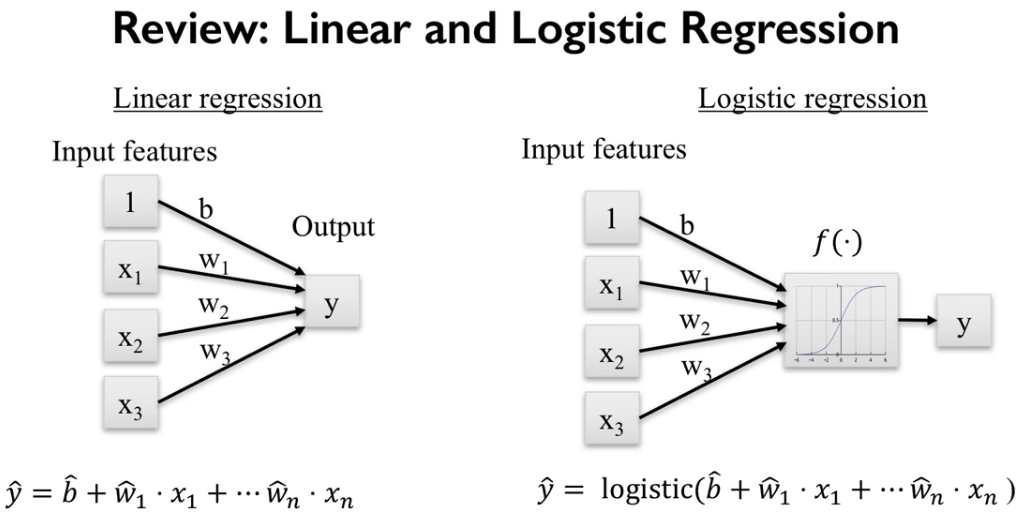
\includegraphics[width=\linewidth]{img/Linear-Regression-Logistic-Regression.png} 
\end{center} 

Linear regression predicts a continuous output, $\hat{y}$, shown as the box on the right. As a function as the sum of the input variables $x_i$, shown in the boxes on the left. 

Each weighted by a corresponding coefficient, $\hat{w}_i$, plus an intercept or bias term, $\hat{b}$. We saw how various methods like ordinary least squares, ridge regression or lasso regression. Could be used to estimate these model coefficients, $\hat{w}_i$, and $\hat{b}$, shown above the arrows in the diagram, from training data. 

Logistic regression takes this one step further, by running the output of the linear function of the input variables, $x_i$. Through an additional nonlinear function, the logistic function. Represented by the new box in the middle of the diagram, to produce the output, $y$. 

Which, because of the logistic function, is now constrained to lie between 0 and 1. 

We use \emph{logistical regression} for \emph{binary classification}. Since we can interpret $y$ as the \emph{probability} that a given input data instance belongs to the positive class, in a two-class binary classification scenario. 

Here's an example of a simple neural network for regression, called a multi-layer perceptron (MLP). These are also known as \emph{feed-forward neural networks}.

\begin{center}
	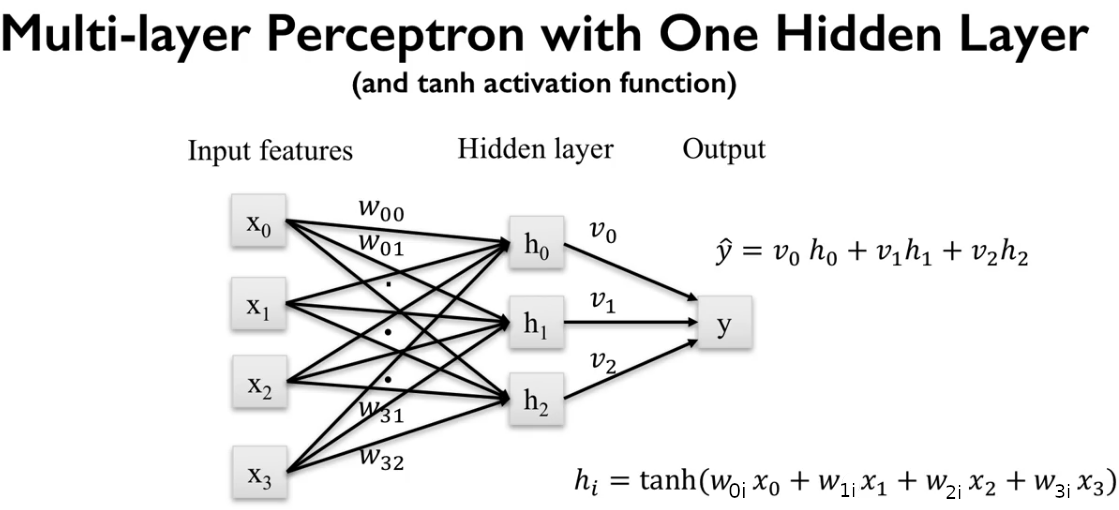
\includegraphics[width=\linewidth]{img/Multi-layer-Perseptron.png} 
\end{center}

MLPs take this idea of computing weighted sums of the input features, like we saw in logistic regression. But it takes it a step beyond logistic regression, by adding an additional processing step called a \emph{hidden layer}. Represented by this additional set of boxes, $h_0$, $h_1$ and $h_2$ in the diagram. These boxes, within the hidden layer, are called \emph{hidden units}. And each hidden unit in the hidden layer computes a \emph{nonlinear} function of the weighted sums of the input features. Resulting in \emph{intermediate} output values, $v_0, v_1, v_2$. Then the MLP computes a weighted sum of these hidden unit outputs, to form the final output value, $\hat{y}$. 

This nonlinear function that the hidden unit applies. is called the \emph{activation function}. In this example, your activation function is the hyperbolic tangent function, which is related to the logistic function. You can see that the result of adding this additional hidden layer processing step to the prediction model, is a formula for $\hat{y}$. That is already more involved than the one for logistic regression. Now predicting $\hat{y}$ involves computing a different initial weighted sum of the input feature values for each hidden unit. Which applies a nonlinear activation function. And then all of these nonlinear outputs are combined, using another weighted sum, to produce $\hat{y}$. 

In particular, there's one weight between each input and each hidden unit. 
And one weight between each hidden unit and the output variable. 

In fact, this addition and combination of non-linear activation functions allows multi-layer perceptrons to learn more complex functions than is possible with a simple linear or logistic function. This additional expressive power enables neural networks to perform more accurate prediction when the relationship between the input and output is itself complex. 

Of course, this complexity also means that there are a lot more weights, model coefficients, to estimate in the training phase. Which means that both \emph{more training data and more computation} are typically needed to learn in a neural network, compared to a linear model. 

As an aside, there are a number of choices for the activation function in a neural network, that gets applied in hidden units. 

\begin{center}
	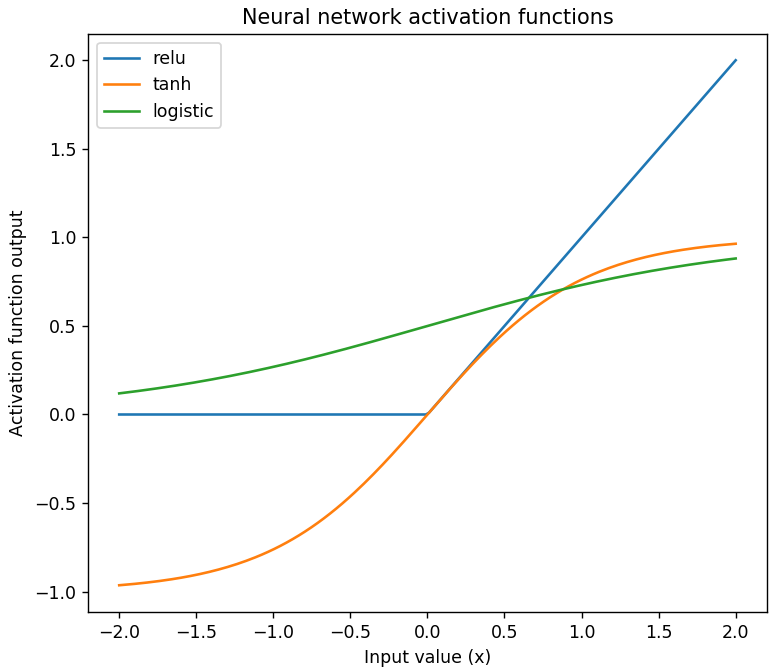
\includegraphics[width=\linewidth]{img/Neural-Network-Activation-Functions.png} 
\end{center}

Here, the plot shows the input value coming into the activation function, from the previous layer's inputs on the x-axis. And the y-axis shows the resulting output value for the function. 

The three main activation functions we'll compare later in this lecture are:
\begin{itemize}
\item the hyperbolic tangent
\item the rectified linear unit function (relu)
\item the logistic function
\end{itemize}

The relu activation function is the default activation function for neural networks in scikit-learn. It maps any negative input values to zero. 

The hyperbolic tangent function, or tanh function maps large positive input values to outputs very close to one. And large negative input values, to outputs very close to negative one. 

These differences in the activation function can have some effect on the shape of regression prediction plots or classification decision boundaries that neural networks learn. 

In general, we'll be using either the hyperbolic tangent or the relu function as our default activation function. Since these perform well for most applications. 

\subsection{Implementation}

Let's take a look at how we use neural networks in scikit-learn for classification. Using the more complex synthetic binary classification data set. 

To use a neural network classifier, you import the MLPClassifier class from the \texttt{sklearn.neural} network module. 

{\scriptsize
\begin{verbatim}
from sklearn.neural_network import MLPClassifier
\end{verbatim}
}

This code example shows the classifier being fit to the training data, using a single hidden layer. With three different numbers of hidden units in the layer, 1 unit, 10 units and 100 units. As with all other classification types we've seen, you can create the classifier objects with the appropriate parameters. And call the fit method on the training data. 

Here, the main parameter for a neural network classifier is this parameter, \texttt{hidden_layer_sizes}. 

This parameter is a list, with one element for each hidden layer, that gives the number of hidden units to use for that layer. So here we're passing a list with a single element. Meaning we want one hidden layer, using the number in the variable called units. 

By default, if you don't specify the \texttt{hidden_layer_sizes} parameter, scikit-learn will create a single hidden layer with 100 hidden units. While a setting of 10 may work well for simple data sets, like the one we use as examples here. For really complex data sets, the number of hidden units could be in the thousands. It's also possible, as we'll see shortly, to create an MLP with more than one hidden layer. By passing a \texttt{hidden_layer_sizes} parameter with multiple entries. 

I want to also note the use of this extra parameter, called \texttt{solver}. Which specifies the algorithm to use for learning the weights of the network. 

Here, we're using the lbfgs algorithm. We'll discuss the \texttt{solver} parameter setting further, at the end of this lecture. 

Also note that we're passing in a \texttt{random_state} parameter, when creating the MLPClassifier object. Like we did for the train-test split function. And we happened to set this \texttt{random_state} parameter to a fixed value of 0. 

This is because for neural networks, their weights are initialized randomly, which can affect the model that is learned. 

Because of this, even without changing the key parameters on the same data set. The same neural network algorithm might learn two different models. Depending on the value of the internal random seed that is chosen. So by always setting the same value for the random seed used to initialize the weights. We can assure the results will always be the same, for everyone using these examples. 

This graphic plots the results of running this code. To show how the number of hidden units in a single layer in the neural network affects the model complexity for classification. 

\begin{center}
	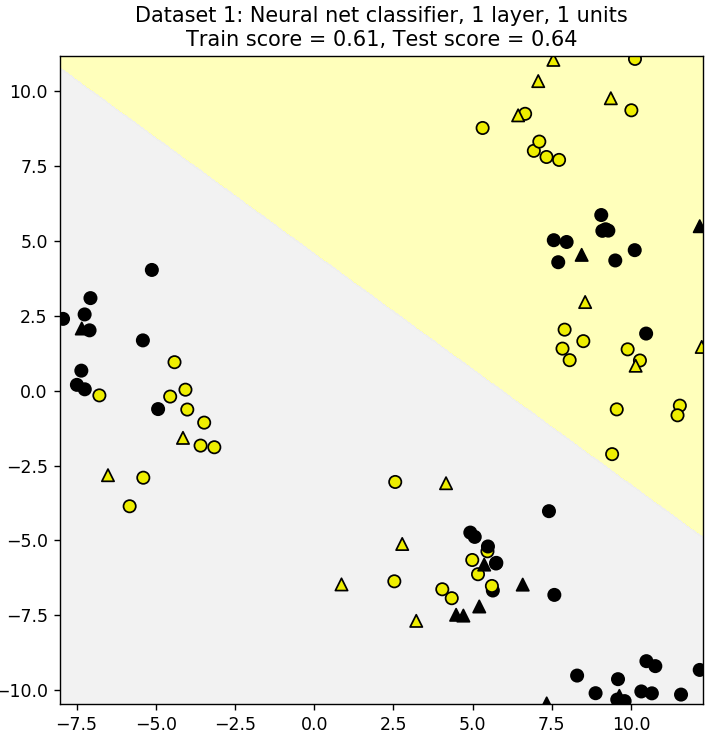
\includegraphics[width=\linewidth]{img/Neural-net-classifier-1layer-1unit.png} 
\end{center}

With 1 hidden unit, the model is mathematically equivalent to logistic regression. We see the classifier returns the familiar simple linear decision boundary between the two classes. The training set score's low, and the test score is not much better, so this network model is under-fitting. 

\begin{center}
	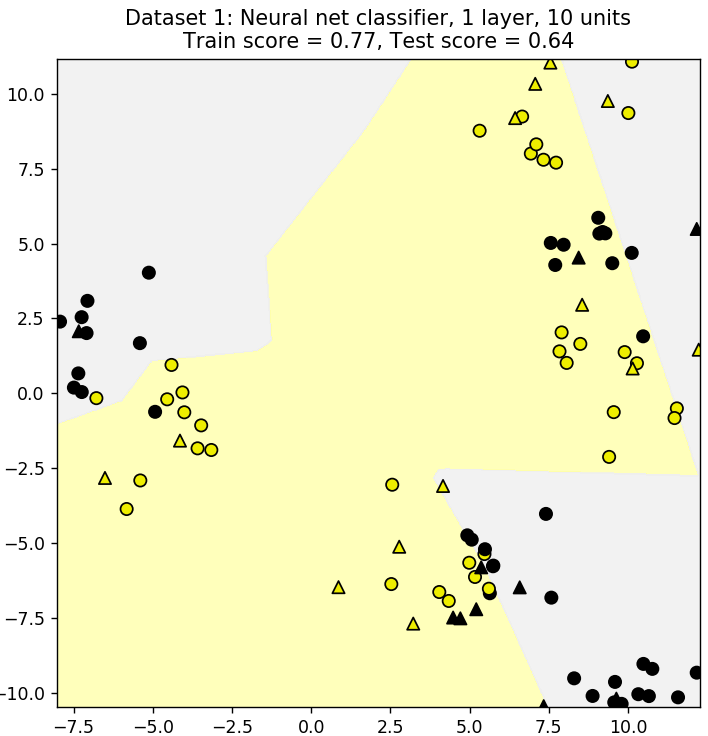
\includegraphics[width=\linewidth]{img/Neural-net-classifier-1layer-10units.png} 
\end{center}

With 10 hidden units, we can see that the MLPClassifier is able to learn a more complete decision boundary. That captures more of the nonlinear, cluster-oriented structure in the data, though the test set accuracy is still low. 

\begin{center}
	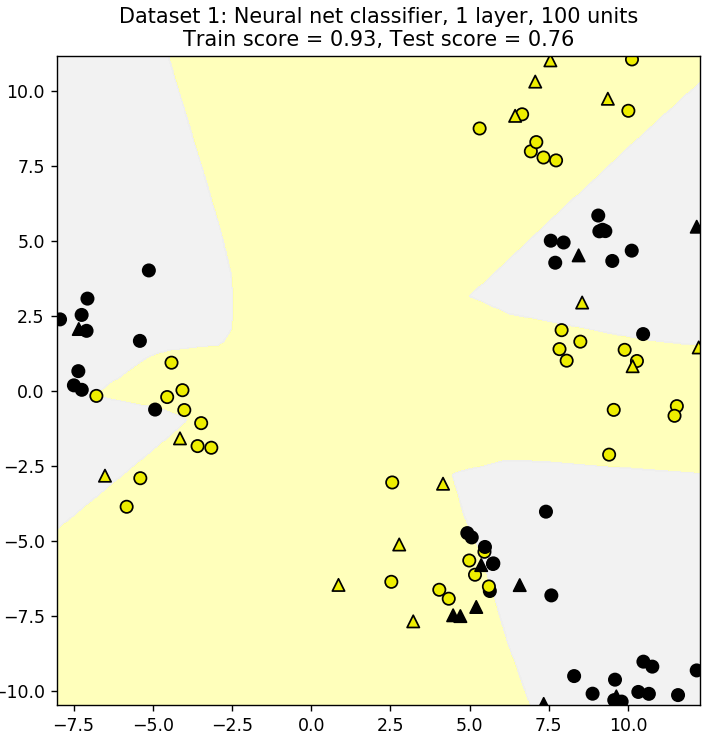
\includegraphics[width=\linewidth]{img/Neural-net-classifier-1layer-100units.png} 
\end{center}

With 100 hidden units, the decision boundary is even more detailed. And achieves much better accuracy, on both the training and the test sets. 

\subsection{Multi-layer Perceptron}

Here's a graphical depiction of a multi-layer perceptron with two hidden layers. 

\begin{center}
	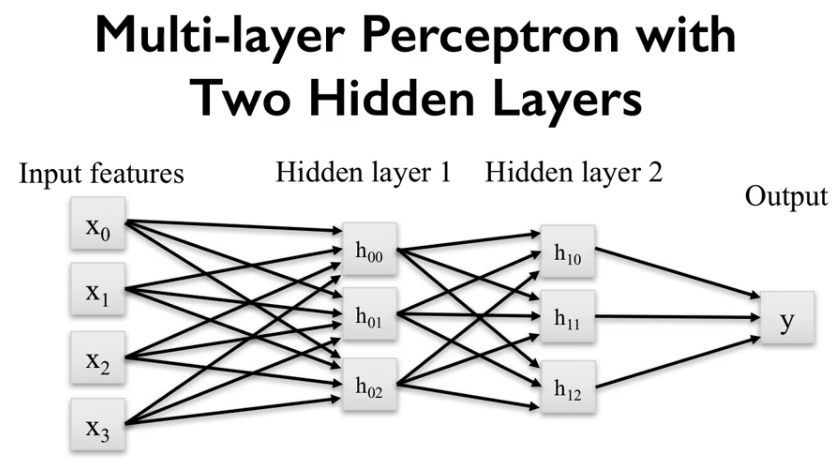
\includegraphics[width=\linewidth]{img/Multi-layer-Perseptron-2Hidden-layers.png} 
\end{center}

Adding the second hidden layer further increases the complexity of functions that the neural network can learn, from more complex data sets. 

Taking this complexity further, large architectures of neural networks, with many stages of computation, are why \emph{deep learning} methods are called deep. 

Here is an example in the notebook, showing how we create a two-layer MLP, with 10 hidden units in each layer. 

{\scriptsize
\begin{verbatim}
nnclf = MLPClassifier(hidden_layer_sizes = [10, 10], 
    solver='lbfgs').fit(X_train, y_train)
\end{verbatim}
}

We just set the \texttt{hidden_layer_sizes} parameter, when creating the MLPClassifier, to a two-element list, indicating ten units, in each of the two hidden layers. 

You can see the result of of adding the second hidden layer, on the classification problem we saw earlier. 

\begin{center}
	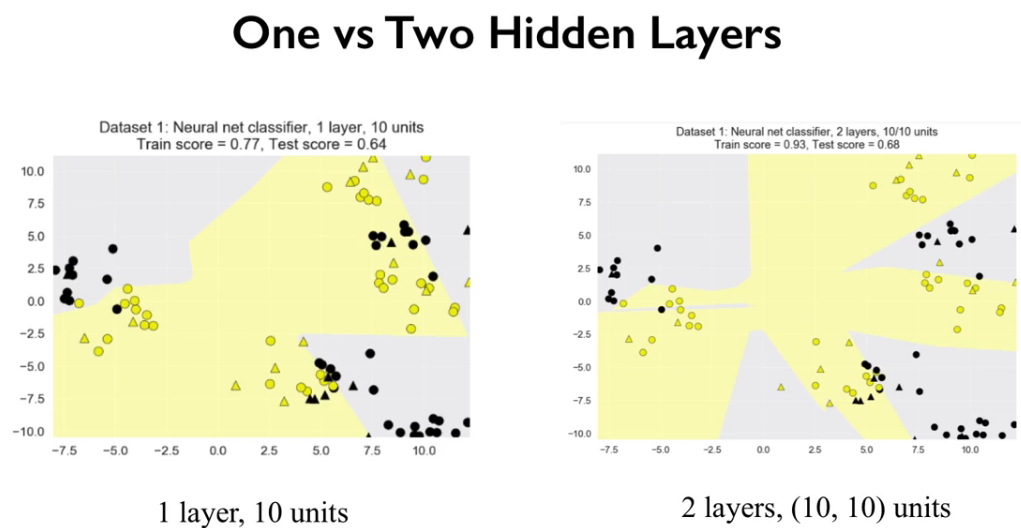
\includegraphics[width=\linewidth]{img/One-vs-Two-Hidden-Layers.png} 
\end{center}

On the left is the original MLP, with one hidden layer of ten units. And on the right is the same data set, using a new MLP with two hidden layers of ten units each. You can see the MLP with two hidden layers learned a more complex decision boundary. And achieved, in this case, a much better fit on the training data, and slightly better accuracy on the test data. 

Once we start adding more hidden layers, with lots of hidden units. You can see that the number of weights, or model coefficients, to estimate for a neural network can increase rapidly. So that more complex neural networks could have many thousands of weights to estimate. 

\subsection{Regularization}

We can control this model complexity, just as we did with ridge and lasso regression, by adding an L2 regularization penalty on the weights. Remember that L2 regularization penalizes models that have a large sum of squares of all the weight values with the effect being that the neural network prefers models with more weights shrunk close to zero. 

The regularization parameter for MLPs is called \texttt{alpha}, like with the linear regression models. And in scikit-learn, it's set to a small value by default, like 0.0001, that gives a little bit of regularization. 

{\scriptsize
\begin{verbatim}
for this_alpha, axis in 
    zip([0.01, 0.1, 1.0, 5.0], subaxes):
    nnclf = MLPClassifier(solver='lbfgs', 
               activation = 'tanh',
               alpha = this_alpha,
               hidden_layer_sizes = [100, 100],
               random_state = 0).fit(X_train, y_train)
\end{verbatim}
}


This code example shows the effects of changing alpha for a larger MLP, with 2 hidden layers of 100 nodes each. From a small value of 0.01, to a larger value of 5.0. For variety here, we're also setting the activation function to use the hyperbolic tangent function. 

Here's the graphical output of this notebook code. You can see the effect of increasing regularization with increasing alpha. 

\begin{center}
	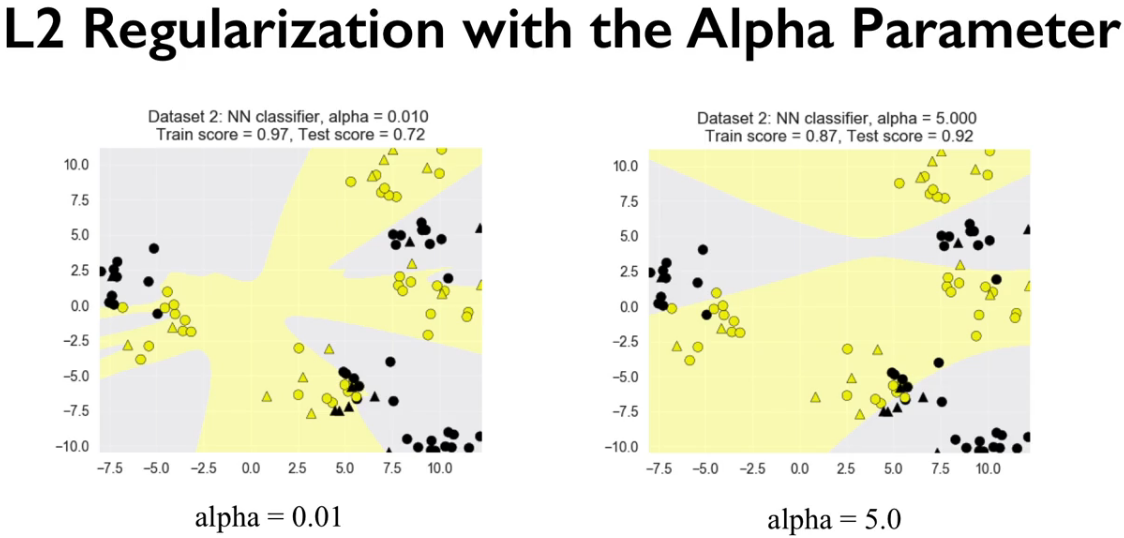
\includegraphics[width=\linewidth]{img/Neural-Network-L2-Regularization.png} 
\end{center}

In the left plot, when alpha is small, the decision boundaries are much more complex and variable. And the classifier's over-fitting, as we can see from the very high training set score, and low test score. On the other hand, the right plot uses the largest value of alpha here, alpha 5.0. And that setting results in much smoother decision boundaries, while still capturing the global structure of the data. And this increased simplicity allows it to generalize much better, and not over-fit to the training set. And this is evident from the much higher test score, in this case. 

\subsection{Features Normalization}

As with other supervised learning models, like regularized regression and support vector machines, it can be \textbf{critical}, when using neural networks, to \emph{properly normalize the input features}. 

Let's apply the multi-layer perceptron to the breast cancer data set. And notice that we first apply the \texttt{MinMaxScaler}, to pre-process the input features. 

Here we'll combine a more complex network, using 2 hidden layers with 100 units each. With a higher regularization setting of alpha at 5.0, and using the lgbfs solver again. 

{\tiny
\begin{verbatim}
from sklearn.neural_network import MLPClassifier
from sklearn.preprocessing import MinMaxScaler

scaler = MinMaxScaler()

X_train, X_test, y_train, y_test = train_test_split(X_cancer, y_cancer,
                                                    random_state = 0)
X_train_scaled = scaler.fit_transform(X_train)
X_test_scaled = scaler.transform(X_test)

clf = MLPClassifier(hidden_layer_sizes = [100, 100], alpha = 5.0,
      random_state = 0, solver='lbfgs').fit(X_train_scaled, y_train)

print('Breast cancer dataset')
print('Accuracy of NN classifier on training set: {:.2f}'
     .format(clf.score(X_train_scaled, y_train)))
print('Accuracy of NN classifier on test set: {:.2f}'
     .format(clf.score(X_test_scaled, y_test)))
     
Breast cancer dataset
Accuracy of NN classifier on training set: 0.98
Accuracy of NN classifier on test set: 0.97 
\end{verbatim}
}

You can see, that with this multi-layer perceptron, both the training and test set accuracy are among the highest we have obtained on this data set. 

\subsection{Regression}

Like many of the other supervised learning methods we've seen, you can also use multi-layer perceptrons for regression, as well as classification. 

We're including MLP regression here, as an example, for two reasons. First, because MLP regression may be useful for some regression problems on its own. But more generally, because some deep learning problems are regression problems. 

And so, as with classification, using multi-layer perceptrons is a good starting point to learn about the more complex architectures used for regression in deep learning. 

{\tiny
\begin{verbatim}
from sklearn.neural_network import MLPRegressor

fig, subaxes = plt.subplots(2, 3, figsize=(11,8), dpi=70)

X_predict_input = np.linspace(-3, 3, 50).reshape(-1,1)

X_train, X_test, y_train, y_test = 
    train_test_split(X_R1[0::5], y_R1[0::5], random_state = 0)

for thisaxisrow, thisactivation in zip(subaxes, ['tanh', 'relu']):
    for thisalpha, thisaxis in zip([0.0001, 1.0, 100], thisaxisrow):
        mlpreg = MLPRegressor(hidden_layer_sizes = [100,100],
                             activation = thisactivation,
                             alpha = thisalpha,
                             solver = 'lbfgs').fit(X_train, y_train)
        y_predict_output = mlpreg.predict(X_predict_input)
        thisaxis.set_xlim([-2.5, 0.75])
        thisaxis.plot(X_predict_input, y_predict_output,
                     '^', markersize = 10)
        thisaxis.plot(X_train, y_train, 'o')
        thisaxis.set_xlabel('Input feature')
        thisaxis.set_ylabel('Target value')
        thisaxis.set_title('MLP regression\nalpha={}, activation={})'
                          .format(thisalpha, thisactivation))
        plt.tight_layout()
\end{verbatim}
}        
        
You use the multi-layer perceptron regressor by importing the MLPRegressor class from the sklearn.neural_network module, and then creating the MLPRegressor object. When creating the object here, we're setting the number of hidden layers and units within each hidden layer. Using the same \texttt{hidden_layer_sizes} parameter that we used for classification. 

This example uses two hidden layers, with 100 hidden nodes each. This notebook code has a loop that cycles through different settings of the \texttt{activation_function} parameter, and the \texttt{alpha} parameter for L2 regularization. 

Here we've included regression results that use, in the top row, the hyperbolic tangent activation function. And in the bottom row, the relu activation function. 


You can see the \emph{smoothness} of the activation function somewhat influences the smoothness of the corresponding regression results. 

Along the columns, the plots also show the effect of using different alpha settings, to increase the amount of L2 regularization from left to right. 

Again, as with classification, the effect of increasing the amount of L2 regularization, by increasing alpha. Is to constrain the regression to use simpler and simpler models, with fewer and fewer large weights. 

You can see this effect for both activation functions, in the top and bottom rows. The regression line on the left has higher variance than the much smoother, regularized model on the right. 

\end{multicols}
\begin{center}
	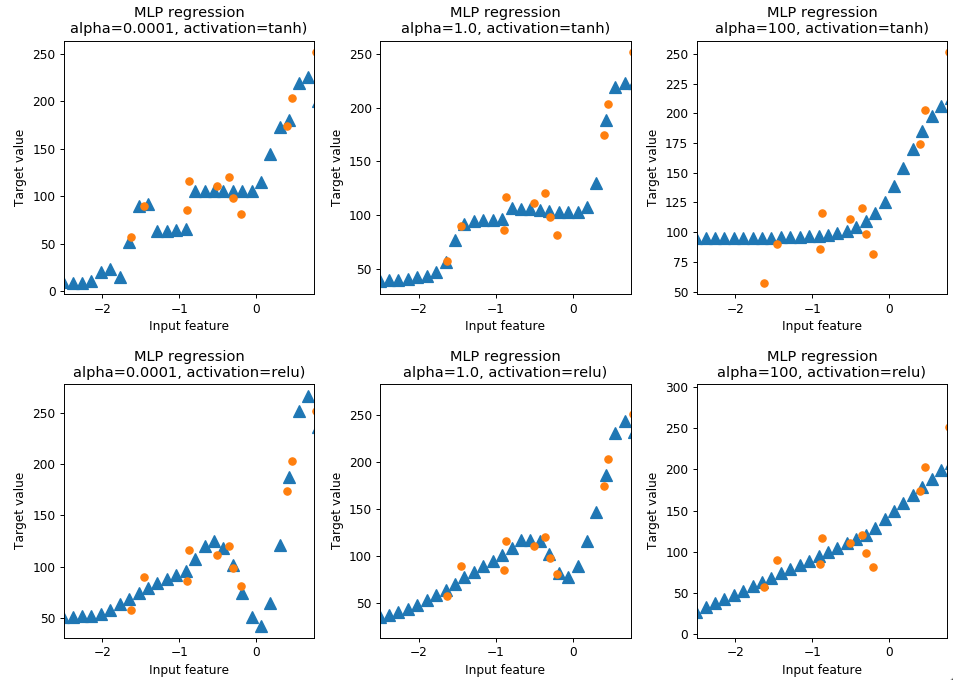
\includegraphics[width=\linewidth]{img/Neural-Networks-Regression.png} 
\end{center}
\begin{multicols}{2}

\subsection{Pros and Cons}

On the positive side, beyond these simple examples we've shown here. Neural networks form the basis of advanced learning architectures. That capture complex features, and give state-of-the-art performance on an increasingly wide variety of difficult learning tasks. 

From world-championship play for the game of Go, to detailed and robust recognition of objects and images. 

However, with this increased power, come increased costs. This larger and more complex models typically \emph{require significant volumes of data, computation, and training time} to learn. 

In addition, \emph{careful pre-processing of the input data} is needed, to help ensure fast, stable, meaningful solutions to finding the optimal set of weights. 

In general, neural networks are a good choice, when the features are of \emph{similar} types. For example, all derived from the pixels of an image. And less of a good choice, when the features are of very different types. 

\subsection{Key Parameters}

Finally, let's review the key parameters for the multi-layer perceptron in scikit-learn, that can be used to control model complexity. 

The main way to control model complexity for the MLP, is to control the hidden unit size and structure. Using the \texttt{hidden_layers_sizes} parameter that controls the number of hidden layers~--- number of elements in list, and the number of units within each layer. Default: \texttt{hidden_layers_sizes = 100}.

\texttt{Alpha} controls the amount of regularization that helps constrain the complexity of the model, by constraining the magnitude of model weights. Default: \texttt{alpha = 0.0001}

Finally, you can experiment with at least three different choices for the nonlinear activation function, by using the \texttt{activation} parameter: \texttt{relu}~--- default, \texttt{logistic} and \texttt{tahn}. 

Earlier, we saw the \texttt{solver} parameter, for specifying the algorithm that learns the network weights. 

\texttt{Solver} is the algorithm that actually does the numerical work of finding the optimal weights. And one intuitive way of visualizing this  process is that all of the solver algorithms have to do a kind of hill-climbing in a very bumpy landscape, with lots of local minima. 

Where each local minimum corresponds to a locally optimal set of weights. That is, a choice of weight setting that's better than any nearby choices of weights. So across this whole landscape of very bumpy local minima. Some will have higher validation scores on the test data, and some will have lower. So depending on the initial random initialization of the weights. And the nature of the trajectory in the search path that a solver takes through this bumpy landscape. The solver can end up at different local minima, which can have different validation scores. 

The default solver, \texttt{adam}, tends to be both efficient and effective on large data sets, with thousands of training examples. 

For \emph{small} data sets, like many of the ones we use in these examples, the \texttt{lbfgs} solver tends to be faster, and find more effective weights.
\end{multicols}